\documentclass[12pt, a4paper, twoside]{article}

% setup for images
\usepackage{graphicx}
\graphicspath{{./images/}}

% for sub figure environment.
\usepackage{subcaption}

\usepackage{xcolor} % for colors used by links etc.

% for math equations and symbols
\usepackage{amsmath}

\usepackage{enumitem}


% Setup the margins
\usepackage[a4paper, hmargin=1in, top=1in, bottom=1in]{geometry}
\usepackage{multirow} % support for multi-row and multi-col tables.
\usepackage{hyperref}
\hypersetup{
    colorlinks=true,
    linkcolor=blue,
    filecolor=magenta,
    urlcolor=red,
    pdftitle={RnD Report-ChandraSekhar} % Need to change this everytime
    }
\urlstyle{same} %url font style same as rest of text. Default is monospace.
    
% Fancy hdr module setup
\usepackage{fancyhdr}
\pagestyle{fancy}
\fancyhf{} % Clear old header and footer that we don't want

% Setup the first page
\title{RnD Endterm Report}
\author{D.Chandra Sekhar \\[4pt] 190050031}
\date{\today}


% Setup the contents on border
\rfoot{Page \thepage}
\lhead{Chandra Sekhar}
\rhead{\leftmark}
\renewcommand{\headrulewidth}{2pt} % default is 1
\renewcommand{\footrulewidth}{1pt} %default is 0

\setlength{\headheight}{14.49998pt}
\begin{document}
\maketitle
\vspace{5cm}
\begin{center}
    {\large \textbf{Topic:} Targeted Subset Selection for Accented Speech Recognition \par}
    \vspace{10pt}
    {\large \textbf{Guide}: Ganesh RamaKrishnan Sir \par}
    \vspace{10pt}
    {\large \textbf{Co-Guide}: Preethi Jyothi Madam \par}
    
\end{center}
\thispagestyle{empty}
\newpage
\tableofcontents
\thispagestyle{empty}
\clearpage

\section{Problem Statement}
\subsection{Idea}
Recent ASR models have achieved good WERs on \textbf{native} English speech. But still they fail to achieve good WERs on \textbf{accented} English speech.
The reason for this is : lack of good representation of accented speech samples in the training data-sets.

One solution for this problem is to just collect more speech samples of the targeted accent and finetune the pretrained model on those samples.
But the limitation is that:  collecting large number of such annotated/transcribed speech samples is expensive.
Hence we seek for solutions which use comparitively lesser number of annotated speech samples.

\subsection{Formal Statement}
\begin{center}
    \begin{tabular}{ |c|c|c| }
        \hline
        \textbf{Name}                           & \textbf{Symbol}                & \textbf{Meaning}                                                  \\
        \hline
        \multirow{2}{*}{\textbf{Target Accent}} & \multirow{2}{*}{$\mathbf{T}$}  & Accent on which we want the ASR model                             \\
                                                &                                & to perform well                                                   \\
        \hline
        \textbf{Target Set}                     & $\mathcal{T}$                  & Unannotated samples from  target accent.                          \\

        \hline
        \multirow{2}{*}{\textbf{Ground Set}}    & \multirow{2}{*}{$\mathcal{G}$} & Collection of large number of unannotated                         \\
                                                &                                & speech samples from various accents.                              \\
        \hline
        \multirow{2}{*}{\textbf{Selected Set}}  & \multirow{2}{*}{$\mathcal{X}$} & $\mathcal{X} \subseteq \mathcal{G}$. Samples which are sent for   \\
                                                &                                & annotation and further used for finetuning.                       \\
        \hline
        \multirow{2}{*}{\textbf{Test Set}}      & \multirow{2}{*}{$\mathcal{Y}$} & Annotated Samples on which our                                    \\
                                                &                                & finetuned model is evaluated.                                     \\
        \hline
        \multirow{2}{*}{\textbf{Budget}}        & \multirow{2}{*}{$\mathcal{B}$} & The maximum duration of speech samples                            \\
                                                &                                & which we can get annotated                                        \\
        \hline
        \textbf{Budget-Constraint}              & $\mathcal{C}$                  & $\sum_{x \in \mathcal{X}}{\mathtt{duration(x)}} \leq \mathcal{B}$ \\
        \hline
    \end{tabular}

\end{center}
Under the above notation, our goal is to propose an algorithm that
selects $\mathcal{X}$ such that, $\mathcal{C}$ is obeyed and the performance
of finetuned model on $\mathcal{Y}$ is maximised.

\vspace{5pt}
To evaluate the performance of our selection($\mathcal{X}$) we define an \textbf{Oracle} performance measure.
It is calculated by sampling $\mathcal{Z}$ from $\mathcal{G}$ randomly s.t. $\mathcal{Z}$ only has samples from $\mathbf{T}$,
annotating them, fine tuning our model on $\mathcal{Z}$ and evaluating finetuned model on $\mathcal{Y}$. 

\vspace{5pt}
Under the experimental setting we actually know the accents of all samples in $\mathcal{G}$. Therefore sampling $\mathcal{Z}$ is
possible. While sampling $\mathcal{X}$ we make sure that we don't use the accent information in any unrealistic way. In the real-world, we may not know accent information for all samples, but this is not a problem
because, we anyway don't need to sample $\mathcal{Z}$ as it is just for checking the performance of our selections. 

\vspace{5pt}
Although this formulation was done from the perspective of Accent-Personalisation, same notation and algorithms
can be applied for Speaker Personalisation setting also.
\clearpage

\section{Algorithm}
\subsection{Idea}
Our goal is to select $\mathcal{X}$ such that samples in $\mathcal{X}$ resemble $\mathbf{T}$ in terms of accent. For this we need an
embedding of speech utterances that preserves the accent information. Once we get these embeddings we need to choose samples $\mathcal{X}$ from $\mathcal{G}$
such that, they are as \textbf{diverse} as possible and as \textbf{relevant} as possible to the target set($\mathcal{T}$). To ensure this
diversity and relevancy(a.k.a. query coverage) we use Sub-Modular-Information(S.M.I) functions.

\vspace{3pt}
So the main challenge left in this method is in:
\vspace{-6pt}
\begin{enumerate}
    \item Choosing the right embeddings that preserve accent information.
          \begin{enumerate}
              \item MFCC features
              \item Accent-Classifer features.
          \end{enumerate}
    \item Choosing the right S.M.I functions that balance the diversity and coverage.
          \begin{enumerate}
              \item FL2MI
              \item GCMI
              \item LogDMI
          \end{enumerate}
\end{enumerate}

\subsection{Prev Work}

Anmol and Mayank have already explored the idea of using MFCC features along with FL2MI,
GCMI, LogDMI in \cite{kothyari2021personalizing}. It was observed that these work really well
for Speaker and Accent Personalisation tasks on data sets such as Indic and L2-Arctic. Using MFCC features, T-SNE plots
obtained showed that speech samples from the same user clustered together very well.

\subsection{Issues}
\begin{itemize}
    \item When MFCC features were applied on Mozilla-Common Voice data set, the T-SNE plots didn't show
          well formed clusters. Each cluster had speech samples from many different accents. This clearly showed that embeddings should
          be improved from the basic MFCC features in such a way that they capture accent-information.
    \item The reason MFCC features worked well with L2-Arctic and Indic data sets is that both these data sets have very
          small number of speakers per accent and the speech samples didn't have noise, loudness variations etc.
          Basically MFCC was capturing speaker features well when there is no noise in the data set and since number of speakers
          per accent is = 1 (in Indic data set) it appeared as if MFCC was doing well on Accent-Identification.
\end{itemize}

\textit{\textbf{This is where my RnD work exactly started. We needed to come up with new embeddings which capture accent
        information well.}}
\clearpage
\section{Work done in RnD}
Our main aim is to find embeddings that capture accent-information well in spite of noise, loudness variations etc.
\subsection{Semi-Supervised Accent Classifier}
\subsubsection{Idea}
First we thought of training an accent-classifier in a Semi-Supervised fashion. We do few iterations where in each iteration we select few utterances based on their current pseudo labels and send them for accent-labelling and transcription. Then we add these to our base training set and retrain our model(ASR + accent classifier) using a joint learning approach. At test time, given a test utterance we can take the last layer values of the accent classifier as the accent embedding of that utterance.
These accent embeddings clearly preserve the accent information. But due to \textbf{difficulty of accent-labelling a speech sample at a later point in time},
this method is difficult to apply in practice.
\subsubsection{Papers read}
\begin{itemize}
    \item \underline{\textbf{Neural SSL for Text Classification}}\cite{sun2020neural} : This paper compares various semi supervised learning approaches for the task of text classification.
    
    Let $\mathcal{U}$ denote in-domain \textbf{unlabelled} data, $\mathcal{D}$ denote in-domain \textbf{labelled} data. First a language model like \texttt{RoBERTa}(which can be initialised from scratch or from an open-domain trained version) is trained on $\mathcal{U}$, which is further fine-tuned on $\mathcal{D}$. 
    
    Student-Teacher model is used to train text classifier. We use the embeddings from language model as inputs to the classifier. Teacher is trained on $\mathcal{D}$ and then is used to assign \textbf{pseudo-labels} to $\mathcal{U}$. Top-K samples from $\mathcal{U}$ w.r.t the confidence of teacher model on them are selected and we denote them as $\mathcal{D'}$. Now we have \underline{several alternatives in training the student model}. Let $\mathcal{T}(\mathcal{X})$ denote pre-training of student model on data set $\mathcal{X}$ and let $\mathcal{F}(\mathcal{X})$ denote fine tuning of it on data set $\mathcal{X}$. 
    
    \underline{\textbf{Alternatives}}:
    \begin{enumerate}
        \item $\mathcal{T}(\mathcal{D'})$ 
        \item $\mathcal{T}(\mathcal{D} + \mathcal{D'}) \mathcal{F}(\mathcal{D})$
        \item $\mathcal{T}(\mathcal{D'}) \mathcal{F}(\mathcal{D})$
    \end{enumerate}
    
    This process of training teacher and then using it to further train a student can be iterated. In the iterative method, student is used initialise the teacher for the next iteration then the teacher is finetuned on $\mathcal{D}$ and the process repeats.
    
    Now among these various alternatives (training language model and training student model) this paper evaluates all of those and the conclusions are as follows.
    
    \underline{\textbf{Conclusion}}:
    \begin{enumerate}
        \item Open domain + in-domain pre-training is best for language model when the model size is very large or the in-domain data is less. 
        \item Under the case of very large ($|\mathcal{U}|$) or smaller language model size, only in-domain pre-training is best for the language model.
        \item Among various pseudo-labelling approaches for training student , $\mathcal{T}(\mathcal{D} + \mathcal{D'})$ works best when $|\mathcal{D}|$ is large and $\mathcal{T}(\mathcal{D} + \mathcal{D'}) \mathcal{F}(\mathcal{D})$ works best otherwise.
        \item When the best pretraining technique is combined with best pseudo-labelling approach, their performance gains add up and lead to an even better model.
    \end{enumerate}
\end{itemize}
\subsection{Supervised Accent Classifier}
\subsubsection{Idea}
Instead of training the accent classifier in a semi-supervised fashion we train it in a fully-supervised fashion. Our Accent Classifier uses pretrained Wav2Vec2.0 as its base model and adds an accent classifier layer on top of it. All layers except the last two layers of Wav2Vec2.0 are frozen. We used Mozilla-Common-Voice(MCV) dataset to train the model. Around 1000 samples each, from 8 different accents are used to train the classifier. 
\vspace{-10pt}
\begin{figure}[h]
    \centering
    \includegraphics{images/classifier.png}
    \caption{Classifier Architecture \protect \footnotemark}
    \label{fig:classifier w2v2}
\end{figure}
\footnotetext{This image is drawn by me for this paper \cite{kothyari2021personalizing}}
\vspace{-10pt}
\subsubsection{Papers Read}
We wanted our classifier to generalise across unseen accents well. i.e. the classifier needs to predict a close-by accent when a sample which does not belong to any of the output accents is given as input. For this we explored Self-Supervised learning, Contrastive loss function based approaches. \cite{han2021supervised}, \cite{deng2021improving}, \cite{jain2018improved}
\subsection{Entropy Based Selections}
Though S.M.I. functions ensure coverage and diversity in the selected set $\mathcal{S}$, they don't \textbf{explicitly} try to select the samples on which our ASR model is most uncertain. But selecting these will help the ASR model to learn quicker using lesser number of  samples. 

So to enforce this, we decided to do second-level selections on top of first level S.M.I. based selections. For this we explored the idea of entropy-based selections.
\subsubsection{Papers-Read}
\begin{itemize}
    \item \underline{\textbf{Data selection for speech recognition}}\cite{wu2007data}: Paper's goal is to select utterances to train an acoustic model, in a sample-efficient manner. It assumes that all the utterances are already transcribed(i.e we work with true-transcripts).
    The proposed method is to select the utterances such that the cumulative distribution over words/phonemes/characters in the selected set is as close as possible to uniform distribution. This objective is rewritten in terms of KL-Divergence and is optimised greedily with no performance guarantees. Author reports that this method achieves WERs close to the model trained on full data.
    
    \item \underline{\textbf{Document Summarization technique for speech subset selection}}: \cite{wei2013using} \\
    This paper formulates subset selection as a monotone sub-modular optimisation problem. Monotone sub-modular functions can be optimised (upto a constant factor from the optimal solution) very efficiently using greedy strategies and moreover this is the best that can be done in $\mathbf{P}$-time. 
    
    This paper investigates \texttt{Facility Location function} and \texttt{Saturated Coverage function} together with the following similarity kernels:
    \begin{itemize} 
        \item \textbf{Fisher Similarity}: This is a purely acoustic similarity measure. Let $\theta_1, \ldots \theta_m$ be the parameters of m-HMM models, then
        \begin{align*}
            U^{\theta}_{X} &= \nabla_{\theta} \mathtt{log}(P(X|\theta) \\
            U^{'}_{X} &= [(U^{\theta_1}_{X})^T, (U^{\theta_2}_{X})^T, \ldots  (U^{\theta_m}_{X})^T]^T \\
            \mathtt{d}_{i,j } &= || U^{'}_i -  U^{'}_j|| \\
            \mathtt{sim}_{i,j} &= (\max_{i', j'} d_{i', j'}) - d_{i,j} \\
        \end{align*}
        \vspace{-1.5cm}
        \item \textbf{TF-IDF weighted cosine similarity}: This is a discrete representation based similarity measure. We first construct pseudo-transcripts of each sentence. Now considering each transcript as a sentence with word being the 3-gram phonemes, we construct their TF-IDF vectors.
        $$sim_{i,j} = \frac{<vec_i, vec_j>}{\sqrt{<vec_i, vec_i> <vec_j, vec_j>}}$$
        \item \textbf{Gapped string kernel}\label{Gapped String Kernel}: This is a discrete representations based similarity measure. Let $\Sigma$ denote the set of phonemes, then $\phi: \Sigma^* \to \mathcal{H}$ is defined as 
        $$
            \phi^k_u(s) := \sum_{\mathbf{i}: u = s(i)} \lambda^{span(i)} , \;\; u \in \Sigma^k
        $$
        
        The summation is over $\mathbf{i}$ which is the set of all sub-sequences over $\{ 1, \ldots |s|\}$. Let $i = \{i_1, i_2, \ldots i_q\}$ then $\mathtt{span}(\mathbf{i}) = i_q - i_1 + 1$. 
        
        \begin{align*}
            \mathcal{K}(s_i, s_j) &= \frac{\sum_u{<\phi^k_u(s_i), \phi^k_u(s_j)>w_u}}{\sqrt{<vec_i, vec_i> <vec_j, vec_j>}}\;\; u \in \Sigma^l
        \end{align*}
        $w_u$ is a weight dependent on the length of u.
        $k, l, \lambda$ are hyper-parameters that are tuned on the validation set. More about the efficient computation and other details can be found here(\cite{rousu2005efficient})
    \end{itemize}
    
    \underline{\textbf{Conclusion}}: Gapped String kernel with facility location S.M.I function works the best and they produce much better results than random, entropy based baselines.  
    
    \item \underline{\textbf{Unsupervised Submodular Subset Selection}} \cite{wei2014unsupervised}: The main contribution of this paper is in coming up with two novel sub modular functions. Then they train an unsupervised model that can produce pseudo-transcripts. Now they work on these pseudo transcripts, using the sub modular functions. For similarity based S.M.I functions, they use Gapped String kernel as similarity measure.
    
    Let $\mathbf{V}$ denote the ground set and $\mathbf{S}$ denote the selected subset, then 
    
    \textbf{Facility Location function}: $$f_{fac}(S) = \sum_{i \in \mathbf{V}} \max_{j \in \mathbf{S}} w_{i,j}$$
    $w_{i,j}$ can be any valid similarity metric . But this paper uses gapped string kernel as similarity measure \ref{Gapped String Kernel}. Facility location functions ensures coverage but may not ensure diversity enough. Hence they introduce \textbf{a novel diversity rewarding} monotonic sub-modular function.
    
    \textbf{Diversity Reward function}: Let $\mathbf{P}_1, \ldots \mathbf{P}_k$ denote disjoint partitions of the ground set. Then 
    $$
        f_{div}(S) = \sum_{n=1}^K{\sqrt{\sum_{j \in P_n \cap S}{\left(\sum_{i \in V}{\frac{w_{i,j}}{|V|}}\right)}}}
    $$
    This function encourages samples to be picked from all the partitions, hence encourages diversity.
    
    To get the benefits of both Facility Location and the Diversity based function, we consider the following S.M.I function
    $$
        f_{fac + div}(S) = \lambda \times f_{div}(S) + (1 - \lambda) \times f_{fac}(S)
    $$
    $\lambda$ is a hyper-parameter that is tuned on validation set.
    
    \underline{\textbf{Issue}}: Both these S.M.I. functions are similarity based. So in order to find the optimal solution, we need to construct a graph, which would make the complexity at least quadratic. So we consider other class of S.M.I. functions, known as \textbf{\textit{feature-based S.M.I functions}}.
    \textbf{Feature Based S.M.I functions}
    \begin{itemize}
        \item \textbf{Basic Idea}:
            $$
                f_{fea}(S) = \sum_{u \in \mathcal{U}} g(m_u(S))
            $$
            Where $\mathcal{U}$ denotes the set of features, $u$ denotes a particular feature, $m_u(S)$ denotes the \textbf{\textit{amount}} of feature in set $S$, g is any concave function like $\mathtt{sqrt}$ .
        \item \textbf{Two-Layer S.M.I function}: Single Layer S.M.I functions enforce coverage of features as they are directly optimising that. But they don't capture redundancy between features. This paper introduces a \textbf{novel two-layer feature based S.M.I function} that can capture redundancy between features.
        
        Let $\mathcal{U}^2$ denote the second level meta-features, $\mathcal{U}^1$ denote the first-level features. Let $|\mathcal{U}^2| = d_2$ and $|\mathcal{U}^1| = d_1$. Let $W\in \mathbf{R}^{d_2 \times d_1}$ be a matrix where $W(u_2, u_1)$ indicates the interaction between $u_2 \in \mathcal{U}^2$ and $u_1 \in \mathcal{U}^1$. Now we define the 2-layer S.M.I function as follows:
        
        $$
            f_{\mathtt{2-fea}} = \sum_{u_2 \in \mathcal{U}^2} g_1\left(\sum_{u_1 \in \mathcal{U}^1}{W(u_2, u_1)g_2(m_{u_1}(S))}\right)
        $$
    \end{itemize}
    \item \underline{\textbf{N-best entropy}}\cite{itoh2012n}: This paper deals with selecting a subset of the data in order to train an acoustic model. It assumes that a baseline model that can produce pseudo-transcripts for all utterances in ground set is already available. The proposed algorithm works on these pseudo-transcripts to do the subset selection. For any speech sample to be useful it needs to satisfy the following two criteria:
    \begin{enumerate}
        \item \textbf{Informativeness}: Adding the sample should make the model learn as much as possible. So the utterances on which our model is least confident are the ones which are most \textit{informative} for our model.
        
        \textbf{Entropy Measure}: Let $u$ be the utterance whose entropy we need to measure. Let  $<s_1, p_1>, <s_2, p_2>, \ldots <s_n, p_n>$ be the top-N transcriptions and their probabilities, $ES_u$ be the entropy score of our acoustic model for utterance $u$.
        $$
            \mathtt{ES_u} = - \sum_{i = 1}^{n}{\left(\left(\frac{p_i}{\sum_{j=1}^{n}{p_j}}\right)\mathtt{log}\left(\frac{p_i}{\sum_{j=1}^{n}{p_j}}\right)\right)}
        $$
        More the value of $\mathtt{ES_u}$ more is its informativeness.
        \item \textbf{Representativeness}: Most of the times it happens that the samples on which our model is least confident are outliers i.e. ones which lie far away from the rest of the training data. According to informativeness these may be highly useful, but in reality they aren't. 
        So to measure representativeness, we first construct n-gram based TF-IDF vectors for each pseudo-transcript and then calculate the distance of each TF-IDF vector from the mean TF-IDF vector where mean is taken over all the samples in the ground set. This distance is used to measure representativeness. Lesser the distance, more is its representativeness.
    \end{enumerate}

    \underline{\textbf{Conclusion}}: Author reports that N-best entropy method beats other confidence based measures. When combined with the representativeness, the method improves even further.
    
    \item \underline{\textbf{Error Driven ASR Personalisation}}\cite{awasthi2021error}: This paper deals with the exact reverse of our problem, Given a ground set of lot of sentences, we try to pick a subset of sentences on which we need to collect the users speech utterance. This paper takes into account the following criteria:
    \begin{enumerate}
        \item \textbf{Informativeness}: To measure informativeness we try to calculate the error that our ASR model would make given an utterance corresponding to that sentence $s$. For this first we convert each grapheme(sentence) into its phonemes using a pre-trained grapheme-phoneme converter, then send these to a model that labels each phoneme with a probability value where the probability indicates the probability that the ASR model would predict that particular phoneme wrongly. 
        
        \item \textbf{Representativeness}: In order to encourage diversity among the selected set, we try to pick sentences which have phonemes that are \textbf{under-represented} in the sentences selected till then.
    \end{enumerate}
\end{itemize}
\subsubsection{Coding-Work}
Most of my coding work is focused on trying out entropy-based techniques on top of first level S.M.I selections, writing helping scripts for the team.

\begin{itemize}
    \item \textbf{\underline{Listening Audio data}}: When our team tried to calculate  WER's of various techniques on the MCV(Mozilla Common Voice) dataset, they've found that pretrained model had very high WERs for Indian and African accents. Indian had WER $\approx$ 90 and African had WER $\approx$ 40. None of the papers that have worked on MCV have reported such results. So in-order to debug this issue, we thought of hearing to those samples manually and checking if the audio samples are really that unclear. \href{https://github.com/ChandraSekhar123331/RnD-Coding-Work/blob/master/Listening_Audio_Samples.ipynb}{Code for this can be found here}.

    \textbf{Conclusion}: African samples are more like U.S samples with better English(in comparison to Indian samples). Also Indian samples had more noise than the African samples, but the noise was not that high. So the WER of around 90 was \textbf{not} justified. Later in a different experiment(about entropy) we observed that the predictions of our pretrained model on Indian samples are grossly incorrect and almost all Indian samples got the exact same wrong prediction. So this made it clear that our data-processing(converting .mp3 to .wav) had issues which led all utterances point to the same .wav file. The issue was in the script that converted all \texttt{.mp3} files to \texttt{.wav} files. Figuring out the pre-processing issue (accidentally :))and fixing it \textbf{is one of my major coding contribution to the project}. 
    
    \item \underline{\textbf{Frame Level Entropy Experiment}}: We decided to implement the idea used in  \cite{itoh2012n} on top of S.M.I selections. But unlike classical models, it is not easy to get top-N predictions from end-to-end deep models. So to get a measure of entropy, we used the following idea: Get the frame level entropy for each frame for the best prediction. Aggregate them using a suitable aggregating function to get the entropy for the utterance. Now we calculate the entropy values, for all the samples selected in the first level S.M.I selections. Then we pick the top-N of them and fine-tune our model on them. If this idea is working, then we should find that the W.E.R of model trained on top-N entropy based samples $<$ W.E.R of model trained on top-N samples based on S.M.I score. \href{https://github.com/ChandraSekhar123331/RnD-Coding-Work/blob/master/entropy.py}{Code for this can be found here}
    
    Unfortunately this didn't turn out to be the case. We tried with different aggregating functions to calculate the aggregated entropy from frame level entropies. We tried mean, median. But none of them worked. 
    
    WER values that we obtained for S.M.I + entropy, only S.M.I are compared \href{https://docs.google.com/spreadsheets/d/1iMZGF6s4Rkus7bDvwN1u_FM12wWA2ujArJ4ZL1ZaZfY/edit#gid=0}{here}.
    
    \item{\underline{\textbf{Correlation between W.E.R and Entropy}}}: As the above experiment didn't work, we tried to find what is wrong with our entropy criterion. For that we checked the correlation between W.E.Rs and the calculated entropies(both w.r.t our pretrained model). If our entropy measure is "really" an uncertainty measure, then we need to see a positive correlation W.E.R and entropy. 
    
    Unfortunately this also did not turn out to be the case. We tried with various aggregating methods like mean, median, mean of top-100, median of top-100 to aggregate the frame level entropies. But in all cases we got almost 0 correlation between W.E.R and the entropy. \href{https://github.com/ChandraSekhar123331/RnD-Coding-Work/blob/master/check_corrln.sh}{Code for this can be found here}.
    
    \begin{figure}[h]
      \centering
      \begin{subfigure}[b]{0.4\linewidth}
        \includegraphics[width=\linewidth]{images/entropy-scatter/output-file-indian-mean-10_mean_10_wer_entropy_scatter.png}
        \caption{Agg = Mean(Top 10 entropies)}
      \end{subfigure}
      \begin{subfigure}[b]{0.4\linewidth}
        \includegraphics[width=\linewidth]{images/entropy-scatter/output-file-indian-median-10_median_10_wer_entropy_scatter.png}
        \caption{Agg = Median(Top 10 entropies)}
      \end{subfigure}
      
      \begin{subfigure}[b]{0.4\linewidth}
        \includegraphics[width=\linewidth]{images/entropy-scatter/output-file-indian-median-20_median_20_wer_entropy_scatter.png}
        \caption{Agg = Median(Top 20 entropies)}
      \end{subfigure}
      \begin{subfigure}[b]{0.4\linewidth}
        \includegraphics[width=\linewidth]{images/entropy-scatter/output-file-indian-median-50_median_50_wer_entropy_scatter.png}
        \caption{Agg = Median(Top 50 entropies)}
      \end{subfigure}
    \end{figure}
    
    Clearly all figures show 0 correlation between aggregated entropy and W.E.R. 
    
    \item \textbf{\underline{Checking if Content-based has any scope}}: As the experiment with entropy based selection failed,  we wanted to check whether content-based selection can have any scope. For this we wanted to compare the W.E.Rs of model finetuned with the following:
    \begin{enumerate}
        \item Selecting \textbf{top-100} samples from S.M.I 800 selections.
        \item Selecting \textbf{random-100} samples from S.M.I 800 selections.
    \end{enumerate}
    If both of them have comparable W.E.Rs then we can expect the content-based selection to have some scope. If top-100 is significantly better than random-100 then we are good with S.M.I 100 itself(which is nothing but top-100 of S.M.I 800). \href{https://github.com/ChandraSekhar123331/RnD-Coding-Work/blob/master/indic-scripts/runner.sh}{Code for this can be found here} and \href{https://github.com/ChandraSekhar123331/RnD-Coding-Work/blob/master/indic-scripts/runner_random.sh}{here}. Results of this experiment can be found in the \href{https://docs.google.com/spreadsheets/d/1Eut6CuPrD-cOcxuAcKcMZC4wSzluujR_MSDu-bSArBY/edit#gid=0}{spreadsheet here}. 
    
    As the results suggest, both S.M.I - 100 and random-100 are comparable. This makes it clear that content-based selection can have some scope. 
    
    \item \textbf{\underline{S.M.I scores for out of domain data}}: Recall that we are doing content-based selection on top of S.M.I selections. So we want the S.M.I selections to select samples whose accent matches with that of target accent and content-based selections filter them and pick the samples that are going to make our model learn the most. As we are doing a two stage selection our budget of S.M.I should be higher now and also we need to take care that even with an increased budget we should not pick out of domain(accent) samples. So we need some signal to identify samples that are from different accent while doing S.M.I selections. For this we investigated if S.M.I scores would provide such a signal. We expected that S.M.I scores drop suddenly once all samples from the current accent are picked. To verify this we plotted graph of S.M.I score(y-axis) and the current serial number(x-axis). \href{https://github.com/ChandraSekhar123331/RnD-Coding-Work/blob/master/indic-scripts/TSS_print_gains.py}{Code for this can be found here}
    
    But the graphs did not show any such sudden drop when all the accents are used in the ground set, which means that S.M.I score can't be used as a signal. But when all the close by accents are removed from the ground-set, the graphs showed steep-decline.
    
    Following are the graphs for \texttt{Accent: Malayalam Male} from Indic dataset.
    \begin{figure}[h]
      \centering
      \begin{subfigure}[b]{0.4\linewidth}
        \includegraphics[width=\linewidth]{images/gains/Mal-Male-logx.png}
        \caption{Close by accents removed. x-axis log scale}
      \end{subfigure}
      \begin{subfigure}[b]{0.4\linewidth}
        \includegraphics[width=\linewidth]{images/gains/Mal-Male-usual-x.png}
        \caption{Close by accents removed. x-axis usual scale}
      \end{subfigure}
      
      \begin{subfigure}[b]{0.4\linewidth}
        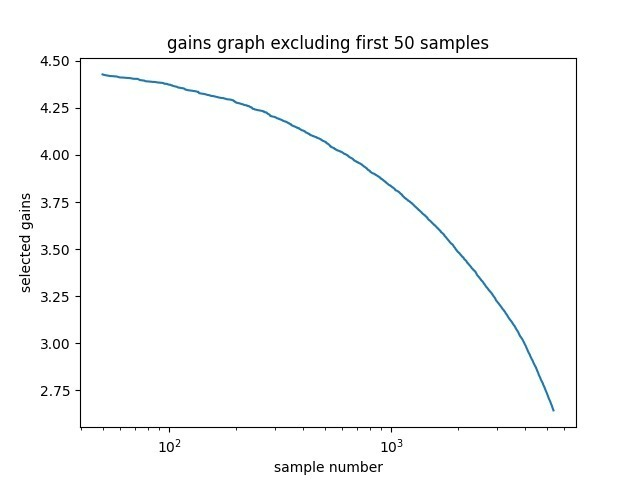
\includegraphics[width=\linewidth]{images/gains/Mal-Male-all-accents-logx.jpeg}
        \caption{All accents. x-axis log scale}
      \end{subfigure}
    \end{figure}
    
    
\end{itemize}



\newpage
\subsection{Misc Papers Read}
\begin{itemize}
    \item \underline{\textbf{QuartzNet}} \cite{kriman2020quartznet} $\&$ \cite{li2019jasper}: We have explored this paper to understand the architecture of QuartzNet better. Primarily we studied about the semantics of output of the model, use of a Language model in the model.
    
    \underline{\textbf{Conclusion}}: QuartzNet is an end-to-end model that does not use any language model. This also helps to compare various ASR models because their performance does not depend on what language model they use. But this obviously comes at the cost of our model making blunder grammatical mistakes when the utterance has noise. Regarding output: QuartzNet outputs a softmax over all the phonemes for each speech-frame.
    
    \item \underline{\textbf{Robust Submodular Observation Selection}} \cite{krause2008robust}: This paper deals with Submodular observation selection under \textbf{multiple constraints}. It gives an algorithm that is at least as good as the optimal set but at a slightly increased budget. Further he proves that we can't do any better than this w.r.t. to the extra budget used. The algorithm is greedy in nature and can be implemented quite efficiently.
    \item Few other papers we referred include: \cite{asami2015training}, \cite{sethy2009iterative}, \cite{woodward2020confidence}
    
    
\end{itemize}




\newpage



\bibliographystyle{IEEEtran}
\bibliography{references}



\end{document}